\documentclass[8pt]{beamer}
\usepackage{ctex}
\usepackage{graphics}
\usepackage{amsmath}
\usepackage{xcolor} 
\usepackage{float}
\usefonttheme[onlymath]{serif}
\usetheme{Warsaw}
%\usecolortheme{dolphin}
\setbeamercovered{transparent}
%%-------------------------------------------------
\title{Weekly Reports}
\author{冯浩哲}

\begin{document}
	\frame{\titlepage}
		
	%%-------------------------------------------------
	
	\section*{Outline}	

\begin{frame}[fragile]
\frametitle{Outline}
\begin{itemize}  
	
\item  The main purpose and the tasks I have finished this week
\vspace{.5cm} 
\item  Things I want to do next week
\vspace{.5cm}
\end{itemize}
\end{frame}

\section*{The main tasks I have finished this week}	
\begin{frame}[fragile]
\frametitle{The main purpose and The tasks I have finished this week}
As last week said,Our main purpose is to build a 3D segmentation network aiming to get a pixel-wise label of the lung node,and to expand suggest annotation technique to 3D space to reduce the burden of label.\\
This week, I mainly read some papers and put effort into tasks above.There are 2 tasks I have finished this week:\\
\vspace{.3cm}
\begin{itemize}
\item Reading some papers about 3D biomedical image segmentation
\vspace{.3cm}
I have read 3 articles about the task.They are \cite{DBLP:journals/corr/KamnitsasLNSKMR16},\cite{DBLP:journals/corr/KayalibayJS17} and \cite{DBLP:journals/corr/RothOHOSFMM17}.\\
\vspace{.3cm}
The first article aims to segment the lesion in brain The net structure is the common FCN,but it raises a efficient training strategy which join the processing of adjacent image patches into one pass through network which can reduce the training burden.\\
\vspace{.3cm}
The second article use the merge operation to improve 3D-Unet,which I want to try in our net in the further experiment.\\
\vspace{.3cm}
The third article also use the common FCN,but it represents a strategy and a loss function which adapt the net into multi-organ segmentation task.
\vspace{.3cm}
\end{itemize}
\end{frame}	

\begin{frame}[fragile]
\frametitle{The tasks I have finished this week}
\vspace{.3cm}
\begin{itemize}
\item Build our net for training 
	\vspace{.3cm}
	I have finished building our net structure as this:
	\begin{figure}[H]
		\centering
		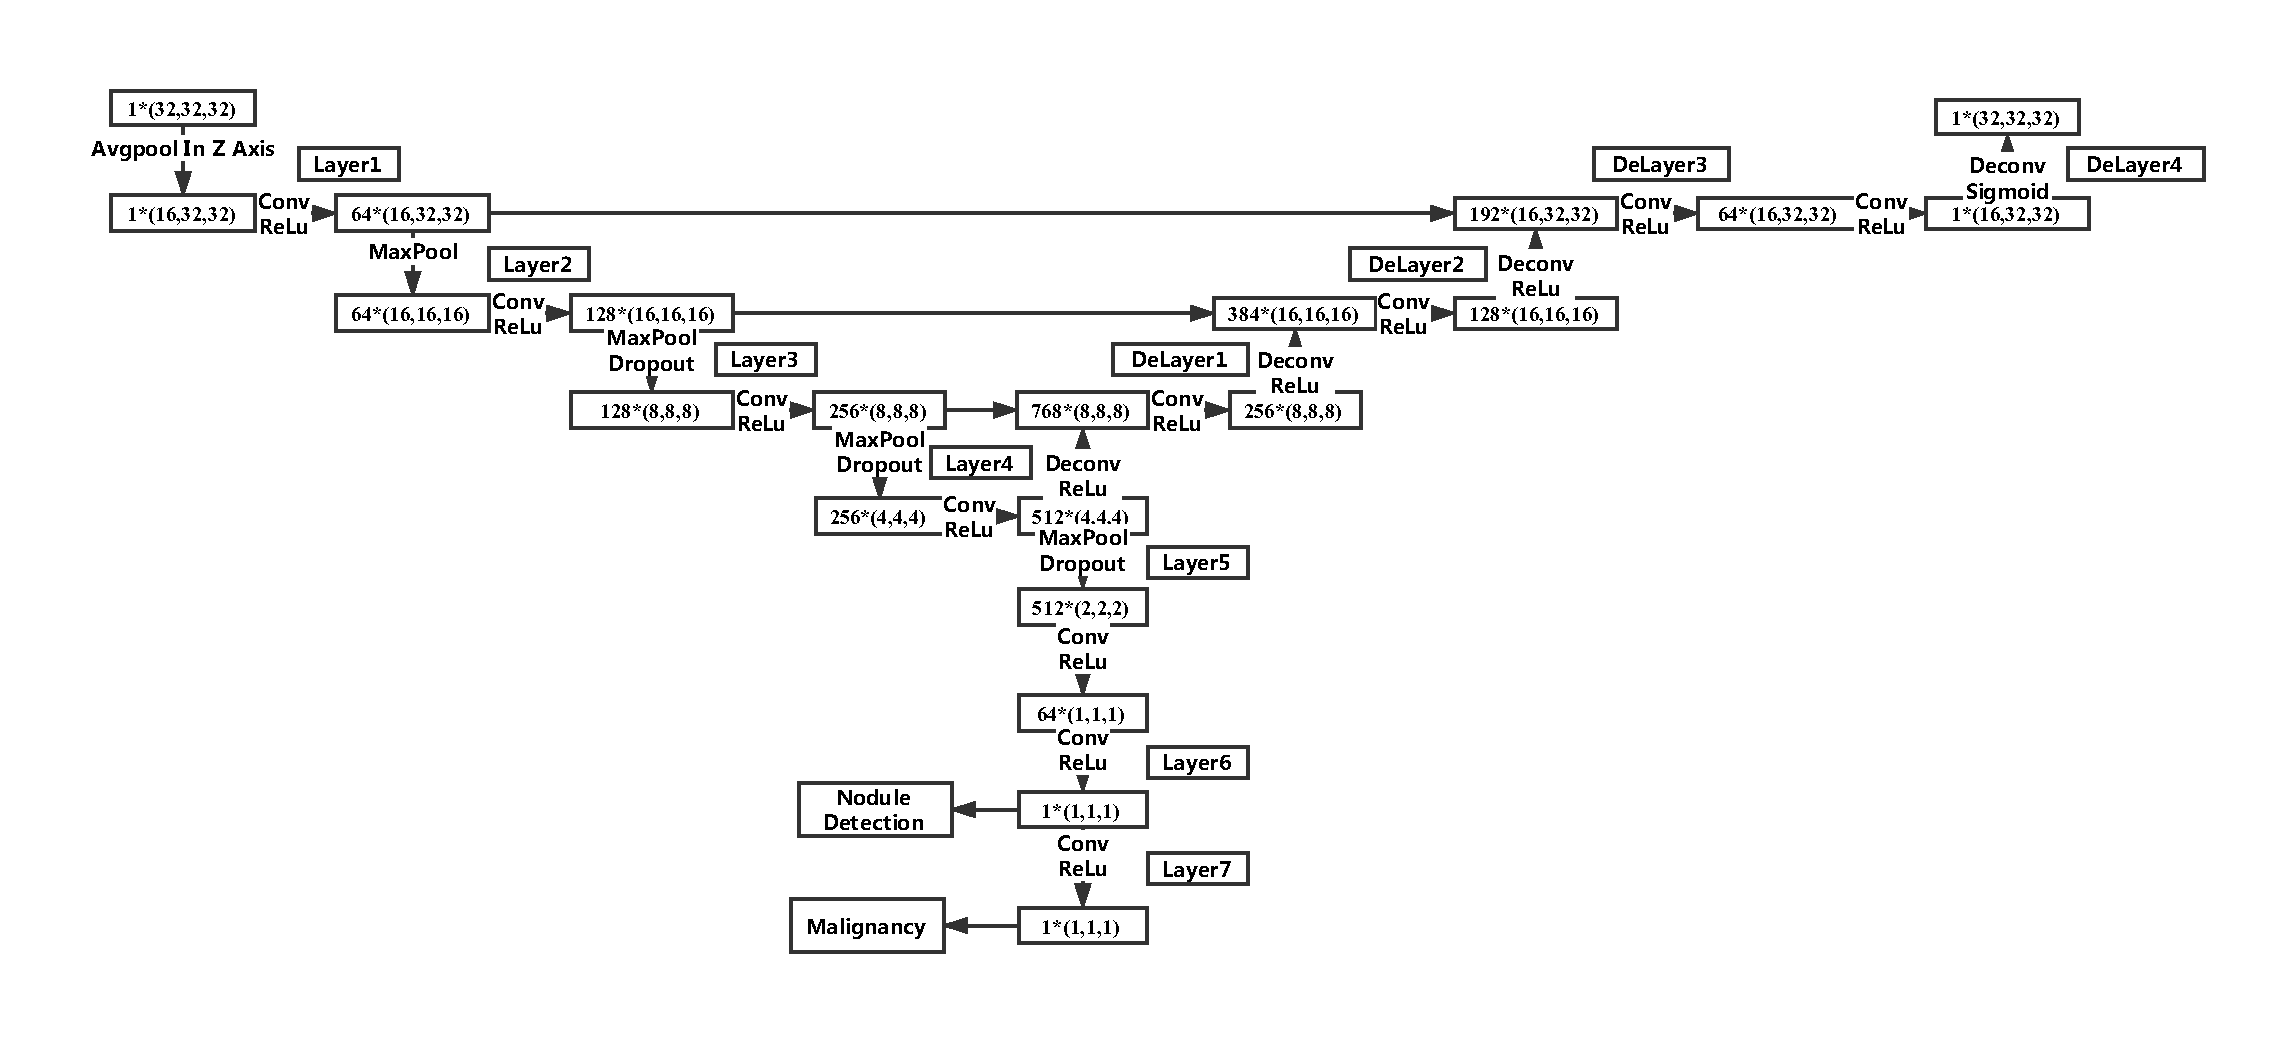
\includegraphics[width=1.0\textwidth]{FirstProject.pdf} 
	\end{figure}
\end{itemize}
\end{frame}

\begin{frame}[fragile]
\frametitle{The tasks I have finished this week}
\vspace{.3cm}
\begin{itemize}
	\item Just as the picture shows,the left half of the net is the same as the 2nd kaggle's structure, and we use part of it into our segment network.
	\vspace{.3cm}
	\item Our train strategy is to train the left part first,and fix the parameter to train the right part until converging.

\end{itemize}
\end{frame}

\begin{frame}[fragile]
\frametitle{The tasks I have finished this week}
\vspace{.3cm}
\begin{itemize}
	\item I also spend 3 days finishing the important but cumbersome task: generating the training data. An example of data is like this :\\
		\begin{figure}[H]
		\centering
		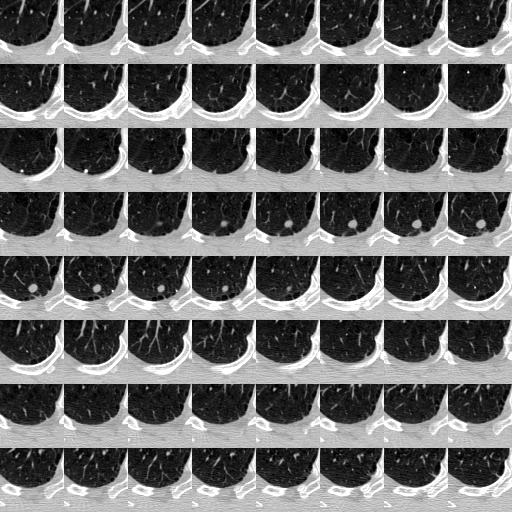
\includegraphics[width=0.5\textwidth]{data.png} 
	\end{figure}
	
	
\end{itemize}
\end{frame}

\begin{frame}[fragile]
\frametitle{The tasks I have finished this week}
\vspace{.3cm}
\begin{itemize}
	\begin{figure}[H]
		\centering
		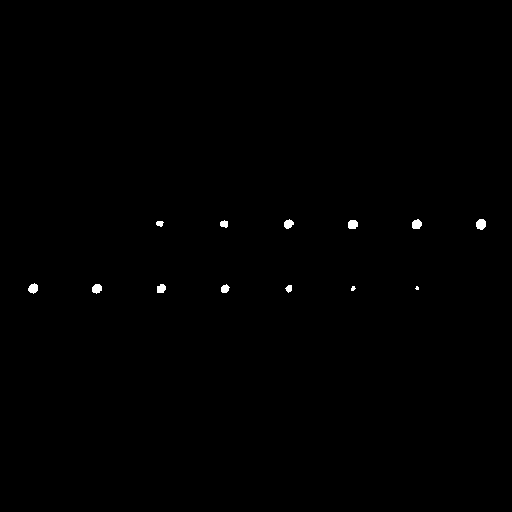
\includegraphics[width=0.5\textwidth]{label.png} 
	\end{figure}
	
	
\end{itemize}
\end{frame}

\section*{Some ideals I want to practice next week}	
\begin{frame}[fragile]
\frametitle{Some ideals I want to practice next week}
Next week, I mainly want to begin the training process of our network.The details of how to load data,how to choose loss function and optimize function is waiting for try.And if our network doesn't work well, I want to use some ideals in the arcticles I mentioned above.
\end{frame}
\bibliography{9_3}
\bibliographystyle{plain}
\end{document}